\lstdefinestyle{base}{
  language=C,
  emptylines=100,
  breaklines=true,
  basicstyle=\ttfamily\color{black},
  moredelim=**[is][\color{darkblue}]{@}{@},
  moredelim=**[is][\color{darkblue}]{***}{***},
}


\lstset{showstringspaces=true,columns=fullflexible,keepspaces=true}

\begin{frame}[fragile]{Beispiel eines invasiven Rust-Programms}

  \begin{center}
    %\vspace*{-2.5cm}
    \only<1>{\includegraphics[width=0.28\textwidth]{images/agentclaim-ex-0.pdf}}
    \only<2>{\includegraphics[width=0.28\textwidth]{images/agentclaim-ex-1.pdf}}
    \only<3,4>{
\includegraphics[width=0.28\textwidth]{images/agentclaim-ex-2.pdf}}
    \only<5>{\includegraphics[width=0.28\textwidth]{images/agentclaim-ex-3.pdf}}
    \only<6,7>{
\includegraphics[width=0.28\textwidth]{images/agentclaim-ex-2.pdf}}
    \only<8>{\includegraphics[width=0.28\textwidth]{images/agentclaim-ex-4.pdf}}
    \only<9-10>{\includegraphics[width=0.28\textwidth]{images/agentclaim-ex-5.pdf}}
    \only<11>{\includegraphics[width=0.28\textwidth]{images/agentclaim-ex-6.pdf}}
    \only<12-13>{\includegraphics[width=0.28\textwidth]{images/agentclaim-ex-5.pdf}}
    \only<14>{
\includegraphics[width=0.28\textwidth]{images/agentclaim-ex-7.pdf}}
    \only<15-16>{\includegraphics[width=0.28\textwidth]{images/agentclaim-ex-8.pdf}}
    \only<17>{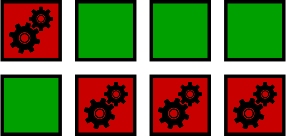
\includegraphics[width=0.28\textwidth]{images/agentclaim-ex-9.pdf}}
    \only<18>{\includegraphics[width=0.28\textwidth]{images/agentclaim-ex-8.pdf}}
    \only<19>{
\includegraphics[width=0.28\textwidth]{images/agentclaim-ex-10.pdf}}
  \end{center}

  \begin{onlyenv}<1>
    \begin{lstlisting}[frame=single,style=base]











    \end{lstlisting}
  \end{onlyenv}

  \begin{onlyenv}<2-3>
    \begin{lstlisting}[frame=single,style=base]
      @let constraints = Constraints::new(4, 8);
      let claim = AgentClaim::new(constraints);@









      \end{lstlisting}
  \end{onlyenv}

  \begin{onlyenv}<4-6>
    \begin{lstlisting}[frame=single,style=base]
      let constraints = Constraints::new(4, 8);
      let claim = AgentClaim::new(constraints);

      @let ilet_fn = |param: *mut c_void| {
        ...
      }
      claim.infect(ilet_fn);@




      \end{lstlisting}
  \end{onlyenv}

  \begin{onlyenv}<7-9>
    \begin{lstlisting}[frame=single,style=base]
      let constraints = Constraints::new(4, 8);
      let claim = AgentClaim::new(constraints);

      let ilet_fn = |param: *mut c_void| {
        ...
      }
      claim.infect(ilet_fn);
      @claim.reinvade(Constraints::new(1, 1));@



      \end{lstlisting}
  \end{onlyenv}

  \begin{onlyenv}<10-12>
    \begin{lstlisting}[frame=single,style=base]
      let constraints = Constraints::new(4, 8);
      let claim = AgentClaim::new(constraints);

      let ilet_fn = |param: *mut c_void| {
        ...
      }
      claim.infect(ilet_fn);
      claim.reinvade(Constraints::new(1, 1));
      @claim.infect(network_fn);@


      \end{lstlisting}
  \end{onlyenv}

  \begin{onlyenv}<13-15>
    \begin{lstlisting}[frame=single,style=base]
      let constraints = Constraints::new(4, 8);
      let claim = AgentClaim::new(constraints);

      let ilet_fn = |param: *mut c_void| {
        ...
      }
      claim.infect(ilet_fn);
      claim.reinvade(Constraints::new(1, 1));
      claim.infect(network_fn);
      @claim.reinvade(Constraints::new(4, 8));@

      \end{lstlisting}
  \end{onlyenv}

  \begin{onlyenv}<16-17>
    \begin{lstlisting}[frame=single,style=base]
      let constraints = Constraints::new(4, 8);
      let claim = AgentClaim::new(constraints);

      let ilet_fn = |param: *mut c_void| {
        ...
      }
      claim.infect(ilet_fn);
      claim.reinvade(Constraints::new(1, 1));
      claim.infect(network_fn);
      claim.reinvade(Constraints::new(4, 8));
      @claim.infect(ilet_fn);@
      \end{lstlisting}
  \end{onlyenv}

  \begin{onlyenv}<18-19>
    \begin{lstlisting}[frame=single,style=base]
      let constraints = Constraints::new(4, 8);
      let claim = AgentClaim::new(constraints);

      let ilet_fn = |param: *mut c_void| {
        ...
      }
      claim.infect(ilet_fn);
      claim.reinvade(Constraints::new(1, 1));
      claim.infect(network_fn);
      claim.reinvade(Constraints::new(4, 8));
      claim.infect(ilet_fn);
      ***// Implizites Retreat beim Verlassen des Geltungsbereichs\end{lstlisting}
  \end{onlyenv}




  

\end{frame}